%%%%%%%%%%%%%%%%%%%%%%%%%%%%%%%%%%%%%%%%%%%%%%%%%%%%%%%%%%%%%%%%%%%%%%%%%%%%
%               feedback-component documentation main.tex                  %
%%%%%%%%%%%%%%%%%%%%%%%%%%%%%%%%%%%%%%%%%%%%%%%%%%%%%%%%%%%%%%%%%%%%%%%%%%%%

\documentclass{report}

\usepackage[margin=1.25in]{geometry}
\usepackage{color}
\usepackage{xcolor}
\usepackage{listings}
\usepackage{caption}
\usepackage{graphicx}
\usepackage{multirow}

\DeclareCaptionFont{white}{\color{white}}
\DeclareCaptionFormat{listing}{\colorbox{gray}{\parbox{\textwidth}{#1#2#3}}}
\captionsetup[lstlisting]{format=listing,labelfont=white,textfont=white}

\renewcommand{\arraystretch}{2.3}

%% rubber: set arguments -shell-escape
\begin{document}
	% TITLE
	\title{Feedback Component API Documentation}
	\author{Martin Ortega}
	\date{\today}
	\maketitle

	% TABLE OF CONTENTS
	\tableofcontents

	% API SERVER
	\chapter{API Server}
		%%%%%%%%%%%%%%%%%%%%%%%%%%%%%%%%%%%%%%%%%%%%%%%%%%%%%%%%%%%%%%%%%%%%%%%%%%%%
%                              api-server.tex                              %
%%%%%%%%%%%%%%%%%%%%%%%%%%%%%%%%%%%%%%%%%%%%%%%%%%%%%%%%%%%%%%%%%%%%%%%%%%%%

\section{Virtual Machine Details}
\begin{center}
\begin{tabular}{|l||p{7cm}|}

\hline
DNS Name         & feedback-api.cloudapp.net             \\
\hline
IP address       & 166.63.215.134                        \\
\hline
Operating System & Ubuntu Server 13.04                   \\
\hline
Size             & Small (1 core @ 1GHz, 1.75 GB memory) \\
\hline
Location         & East Asia                             \\
\hline
Open Ports       & 22, 80                                \\
\hline

\end{tabular}
\end{center}


	% MESSAGE AUTHENTICATION
	\chapter{Message Authentication}
		%%%%%%%%%%%%%%%%%%%%%%%%%%%%%%%%%%%%%%%%%%%%%%%%%%%%%%%%%%%%%%%%%%%%%%%%%%%%
%                        message-authentication.tex                        %
%%%%%%%%%%%%%%%%%%%%%%%%%%%%%%%%%%%%%%%%%%%%%%%%%%%%%%%%%%%%%%%%%%%%%%%%%%%%

\section{HMAC-SHA-1}

For the request authentication portion of the feedback API, we're using the HMAC SHA-1
algorithm. The algorithm works as follows. The client and server share a secret key.
Whenever the client sends a request to the server they compute the SHA-1 hash value of
a certain portion of the request using the secret key and they include that hash value
as one of the request headers. When the server receives a request, they use the same
algorithm to compute what the hash value for the request should be. If the expected hash
doesn't match the hash sent in the request then the authentication step fails, otherwise
it passes. The hash values will be different if either the secret key is not the same
for both sides, or the algorithm is not exactly the same. Here is an image that depicts
the algorithm:

\vspace{1cm}

\begin{center}
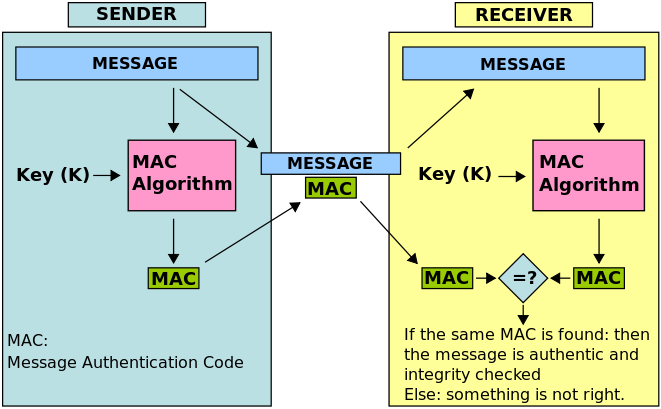
\includegraphics[width=0.8\textwidth]{HMAC_Explanation.png}
\end{center}


%%%%%%%%%%%%%%%%%%%%%%%%%%%%%%%%%%%%%%%%%%%%%%%%%%%%%%%%%%%%%%%%%%%%%%%%%%%%

\section{How to Sign a Request}

For all requests, the server expects to find the request signature in the \\
\textbf{\textit{Feedback-Component-HMAC-SHA-1~}}
header variable. For the examples in the following sections assume that the
secret key is the string 'secret key'.

\subsection{GET and DELETE Requests}

For GET and DELETE requests, the hash value is computed from the concatenation
of the http verb, resource path, and query string in that order.
\subsubsection{Examples}

\begin{center}
\begin{tabular}{|l||l|}

\hline
\multicolumn{2}{|c|}{\textbf{Get Feedback List}} \\
\hline
\textbf{HTTP Verb}                  & GET \\
\hline
\textbf{Resource Path}              & /ichiba/win8/feedback \\
\hline
\textbf{Query}                      & ?minScore=3 \\
\hline
\textbf{Data that should be Hashed} & GET/ichiba/win8/feedback?minScore=3 \\
\hline
\textbf{Hash Signature}             & 81e5913c6757e03d4db7af14bc9dff44a0deca95 \\
\hline

\end{tabular}
\end{center}

\subsection{POST and PUT Requests}
For POST and PUT requests the hash value is computed from the concatenation
of the http verb, resource path, query, and request body in that order.

\subsubsection{Examples}

\begin{center}
\begin{tabular}{|l||l|}

\hline
\multicolumn{2}{|c|}{\textbf{Create Feedback Record}} \\
\hline
\textbf{HTTP Verb}                  & POST \\
\hline
\textbf{Resource Path}              & /ichiba/win8/feedback \\
\hline
\textbf{Query}                      & N/A \\
\hline
\textbf{Body}                       & \{"hello":"world"\} \\
\hline
\textbf{Data that should be Hashed} & POST/ichiba/win8/feedback\{"hello":"world"\} \\
\hline
\textbf{Hash Signature}             & 0a5cb6a2c36c713dfbd57777c751807f5233f481 \\
\hline

\end{tabular}
\end{center}

\begin{center}
\begin{tabular}{|l||l|}

\hline
\multicolumn{2}{|c|}{\textbf{Create User}} \\
\hline
\textbf{HTTP Verb}                  & POST \\
\hline
\textbf{Resource Path}              & /ichiba/win8/users \\
\hline
\textbf{Query}                      & N/A \\
\hline
\textbf{Body}                       & \{\} \\
\hline
\textbf{Data that should be Hashed} & POST/ichiba/win8/users\{\} \\
\hline
\textbf{Hash Signature}             & c94d478f159ba92ca55e51595e95006e8e088ca2 \\
\hline

\end{tabular}
\end{center}



	% API OVERVIEW
	\chapter{API Overview}
		%%%%%%%%%%%%%%%%%%%%%%%%%%%%%%%%%%%%%%%%%%%%%%%%%%%%%%%%%%%%%%%%%%%%%%%%%%%%
%                             api-overview.tex                             %
%%%%%%%%%%%%%%%%%%%%%%%%%%%%%%%%%%%%%%%%%%%%%%%%%%%%%%%%%%%%%%%%%%%%%%%%%%%%

\section{Quick API Overview}

\begin{tabular}{ |c||l||c||p{4cm}| }
\hline

Application Info & /applications & GET & Get a list of all tracked applications and their platforms. \\

\hline
\hline

\multirow{5}{*}{Feature Requests}
&
\multirow{3}{*}{/\$\{app\}/\$\{platform\}/feature\_requests}
& POST & Create a new feature request. \\
\cline{3-4}
&& GET & Get a list of all feature requests for a specific application and platform \\
\cline{2-4}
& /\$\{app\}/\$\{platform\}/feature\_requests/\$\{id\}/votes
& POST & Increment the vote count for a specific feature request \\

\hline
\hline

\multirow{5}{*}{Feedback}
&
\multirow{3}{*}{/\$\{app\}/\$\{platform\}/feeedback}
& POST & Create a new feedback record. \\
\cline{3-4}
&& GET & Get a list of all feedback for a specific application and platform. \\
\cline{2-4}
& /\$\{app\}/\$\{platform\}/feedback/histogram
& GET & Get a histogram of rating score counts. \\

\hline
\hline

Users & /\$\{app\}/\$\{platform\}/users
& POST & Create a new user for a specific application and platform \\

\hline
\end{tabular}


	% APPLICATIONS AND PLATFORMS
	\chapter{Application Info}
		%%%%%%%%%%%%%%%%%%%%%%%%%%%%%%%%%%%%%%%%%%%%%%%%%%%%%%%%%%%%%%%%%%%%%%%%%%%%
%                           application-info.tex                           %
%%%%%%%%%%%%%%%%%%%%%%%%%%%%%%%%%%%%%%%%%%%%%%%%%%%%%%%%%%%%%%%%%%%%%%%%%%%%


%%%%%%%%%%%%%%%%%%%%%%%%%%%%%%%%%%%%%%%%%%%%%%%%%%%%%%%%%%%%%%%%%%%%%%%%%%%%

\section{API Calls}
\begin{center}
\begin{tabular}{|l||l||l|}
\hline

\multicolumn{1}{|c||}{\textbf{API Call}} &
\multicolumn{1}{c||}{\textbf{HTTP Method}} &
\multicolumn{1}{c|}{\textbf{URI}} \\

\hline
\hline
get application and platform list  & GET & /applications \\
\hline
\end{tabular}
\end{center}

%%%%%%%%%%%%%%%%%%%%%%%%%%%%%%%%%%%%%%%%%%%%%%%%%%%%%%%%%%%%%%%%%%%%%%%%%%%%

\section{Get Application and Platform List}

Returns a list of all tracked applications and their respective platforms.
An application and platform are assumed to be in the system if there exists
at least one user for that application and platform.

\subsection{Request Format}
\begin{center}
\begin{tabular}{|l||l|}
\hline
HTTP Method & GET           \\
\hline
URI         & /applications \\
\hline
Query Parameters & N/A       \\
\hline
Body        & N/A            \\
\hline
\end{tabular}
\end{center}

%%%%%%%%%%%%%%%%%%%%%%%%%%%%%%%%%%%%%%%%%%%%%%%%%%%%%%%%%%%%%%%%%%%%%%%%%%%%

\subsection{Response Format}

The response body for this API call is a JSON object with a single field, \textbf{applications},
which is a list of application objects. Every application object has two fields, \textbf{name},
and \textbf{platforms}. The \textbf{name} field is the name of the appliction, and the
\textbf{platforms} field is a list of all platforms that the application has users for.

\vspace{3cm}

%%%%%%%%%%%%%%%%%%%%%%%%%%%%%%%%%%%%%%%%%%%%%%%%%%%%%%%%%%%%%%%%%%%%%%%%%%%%

\subsection{Examples}

\subsubsection{Request}
\textbf{GET} http://feedback-api.cloudapp.net/applications

\subsubsection{Response}
\begin{verbatim}
{
    "applications":[
        {
            "name":"employee_app",
            "platforms":[
                "ios",
                "android"
            ]
        },
        {
            "name":"ichiba",
            "platforms":[
                "win8",
                "web",
                "ios",
                "android"
            ]
        },
        {
            "name":"approval_app",
            "platforms":[
                "ios"
            ]
        }
    ]
}
\end{verbatim}


	% FEATURE REQUESTS
%	\chapter{Feature Requests}
%		%%%%%%%%%%%%%%%%%%%%%%%%%%%%%%%%%%%%%%%%%%%%%%%%%%%%%%%%%%%%%%%%%%%%%%%%%%%%
%                           feature-resuests.tex                           %
%%%%%%%%%%%%%%%%%%%%%%%%%%%%%%%%%%%%%%%%%%%%%%%%%%%%%%%%%%%%%%%%%%%%%%%%%%%%

\section{API Calls}
\begin{center}
\begin{tabular}{|l||l||l|}
\hline

\multicolumn{1}{|c||}{\textbf{API Call}} &
\multicolumn{1}{c||}{\textbf{HTTP Method}} &
\multicolumn{1}{c|}{\textbf{URI}} \\

\hline
\hline
create feature request   & POST & /\$\{app\}/\$\{platform\}/feature\_requests                \\
\hline
get feature request list & GET  & /\$\{app\}/\$\{platform\}/feature\_requests                 \\
\hline
increment vote count     & POST & /\$\{app\}/\$\{platform\}/feature\_requests/\$\{id\}/votes \\
\hline
\end{tabular}
\end{center}

%%%%%%%%%%%%%%%%%%%%%%%%%%%%%%%%%%%%%%%%%%%%%%%%%%%%%%%%%%%%%%%%%%%%%%%%%%%%

\section{Create Feature Request}

Creates a feature request record.

%%%%%%%%%%%%%%%%%%%%%%%%%%%%%%%%%%%%%%%%%%%%%%%%%%%%%%%%%%%%%%%%%%%%%%%%%%%%

\subsection{Request Format}

%%%%%%%%%%%%%%%%%%%%%%%%%%%%%%%%%%%%%%%%%%%%%%%%%%%%%%%%%%%%%%%%%%%%%%%%%%%%

\subsection{Response Format}

%%%%%%%%%%%%%%%%%%%%%%%%%%%%%%%%%%%%%%%%%%%%%%%%%%%%%%%%%%%%%%%%%%%%%%%%%%%%

\subsection{Examples}

%%%%%%%%%%%%%%%%%%%%%%%%%%%%%%%%%%%%%%%%%%%%%%%%%%%%%%%%%%%%%%%%%%%%%%%%%%%%

\section{Get Feature Request List}

%%%%%%%%%%%%%%%%%%%%%%%%%%%%%%%%%%%%%%%%%%%%%%%%%%%%%%%%%%%%%%%%%%%%%%%%%%%%

\subsection{Request Format}

%%%%%%%%%%%%%%%%%%%%%%%%%%%%%%%%%%%%%%%%%%%%%%%%%%%%%%%%%%%%%%%%%%%%%%%%%%%%

\subsection{Response Format}

%%%%%%%%%%%%%%%%%%%%%%%%%%%%%%%%%%%%%%%%%%%%%%%%%%%%%%%%%%%%%%%%%%%%%%%%%%%%

\subsection{Examples}

%%%%%%%%%%%%%%%%%%%%%%%%%%%%%%%%%%%%%%%%%%%%%%%%%%%%%%%%%%%%%%%%%%%%%%%%%%%%

\section{Increment Vote Count}

%%%%%%%%%%%%%%%%%%%%%%%%%%%%%%%%%%%%%%%%%%%%%%%%%%%%%%%%%%%%%%%%%%%%%%%%%%%%

\subsection{Request Format}

%%%%%%%%%%%%%%%%%%%%%%%%%%%%%%%%%%%%%%%%%%%%%%%%%%%%%%%%%%%%%%%%%%%%%%%%%%%%

\subsection{Response Format}

%%%%%%%%%%%%%%%%%%%%%%%%%%%%%%%%%%%%%%%%%%%%%%%%%%%%%%%%%%%%%%%%%%%%%%%%%%%%

\subsection{Examples}


	% FEEDBACK
	\chapter{Feedback}
		%%%%%%%%%%%%%%%%%%%%%%%%%%%%%%%%%%%%%%%%%%%%%%%%%%%%%%%%%%%%%%%%%%%%%%%%%%%%
%                               feedback.tex                               %
%%%%%%%%%%%%%%%%%%%%%%%%%%%%%%%%%%%%%%%%%%%%%%%%%%%%%%%%%%%%%%%%%%%%%%%%%%%%

\section{API Calls}
\begin{center}
\begin{tabular}{|l||l||l|}
\hline

\multicolumn{1}{|c||}{\textbf{API Call}} &
\multicolumn{1}{c||}{\textbf{HTTP Method}} &
\multicolumn{1}{c|}{\textbf{URI}} \\

\hline
\hline
create feedback        & POST & /\$\{app\}/\$\{platform\}/feedback                   \\
\hline
get feedback list      & GET  & /\$\{app\}/\$\{platform\}/feedback                    \\
\hline
get feedback histogram & GET  & /\$\{app\}/\$\{platform\}/feedback/\$\{id\}/histogram \\
\hline
\end{tabular}
\end{center}

\section{Create Feedback Record}

Creates a feedback record for a spefic app and platform.

\subsection{Request Format}

\begin{center}
\begin{tabular}{|l||l|}
\hline
HTTP Method & POST           \\
\hline
URI         & /\$\{app\}/\$\{platform\}/feedback \\
\hline
Query Parameters & N/A           \\
\hline
Body        & TODO           \\
\hline
\end{tabular}
\end{center}


\subsection{Response Format}

\section{Get Feedback List}

Gets a list of all feedback records for a specific app and platform. The
feedback list can optionally filtered by app version, page the feedback was
submitted from, score, and date.

\subsection{Request Format}

\begin{center}
\begin{tabular}{|l||l|}
\hline
HTTP Method & GET           \\
\hline
URI         & /\$\{app\}/\$\{platform\}/feedback \\
\hline
Query Parameters & TODO           \\
\hline
Body        & N/A           \\
\hline
\end{tabular}
\end{center}

\subsection{Response Format}

\section{Get Feedback Histogram}

Get feedback score histogram for a specific app and platform. The return object
is a dictionary object that maps score level to the number of users that
rated the app at that score level. The feedback records used to make the
histogram can be filtered by the page the user was on when they submitted
their feedback, the app version, and date range.

\subsection{Request Format}

\begin{center}
\begin{tabular}{|l||l|}
\hline
HTTP Method & GET           \\
\hline
URI         & /\$\{app\}/\$\{platform\}/feedback/histogram \\
\hline
Query Parameters & TODO           \\
\hline
Body        & N/A           \\
\hline
\end{tabular}
\end{center}

\subsection{Response Format}


	% USERS
	\chapter{Users}
		%%%%%%%%%%%%%%%%%%%%%%%%%%%%%%%%%%%%%%%%%%%%%%%%%%%%%%%%%%%%%%%%%%%%%%%%%%%%
%                                 users.tex                                %
%%%%%%%%%%%%%%%%%%%%%%%%%%%%%%%%%%%%%%%%%%%%%%%%%%%%%%%%%%%%%%%%%%%%%%%%%%%%

\section{API Calls}
\begin{center}
\begin{tabular}{|l||l||l|}
\hline

\multicolumn{1}{|c||}{\textbf{API Call}} &
\multicolumn{1}{c||}{\textbf{HTTP Method}} &
\multicolumn{1}{c|}{\textbf{URI}} \\

\hline
\hline
create user   & POST & /\$\{app\}/\$\{platform\}/users                \\
\hline
\end{tabular}
\end{center}

\section{Create User}

Creates a user record for a given application and platform.

\subsection{Request Format}

\begin{center}
\begin{tabular}{|l||l|}
\hline
HTTP Method & POST           \\
\hline
URI         & /\$\{app\}/\$\{platform\}/users \\
\hline
Query Parameters & N/A           \\
\hline
Body        & N/A           \\
\hline
\end{tabular}
\end{center}


\subsection{Response Format}

The response body is a JSON object with a single field, \textbf{user},
which is an object that represents the user record that was just created.
The \textbf{user} object contains four fields;
\begin{center}
\begin{tabular}{l|l}
\textbf{Field} & \textbf{Significance} \\
\hline \\

app & the name of the app the user is linked to \\
platform & the platform the users is using the app on \\
timestamp & the time and date the user record was created \\
\_id & an identifier that can be used to uniquely identify the user record

\end{tabular}
\end{center}

\subsection{Examples}

\textbf{POST} http://feedback-api.cloudapp.net/ichiba/win8/users
\begin{verbatim}
{
    "user":{
        "app":"ichiba",
        "platform":"win8",
        "timestamp":"2013-08-08T01:00:10.924Z",
        "_id":"5202ed9a82e1069944000001"
    }
}
\end{verbatim}


\end{document}
